\documentclass{standalone}
\usepackage{tikz}
\usetikzlibrary{patterns, positioning}


\begin{document}
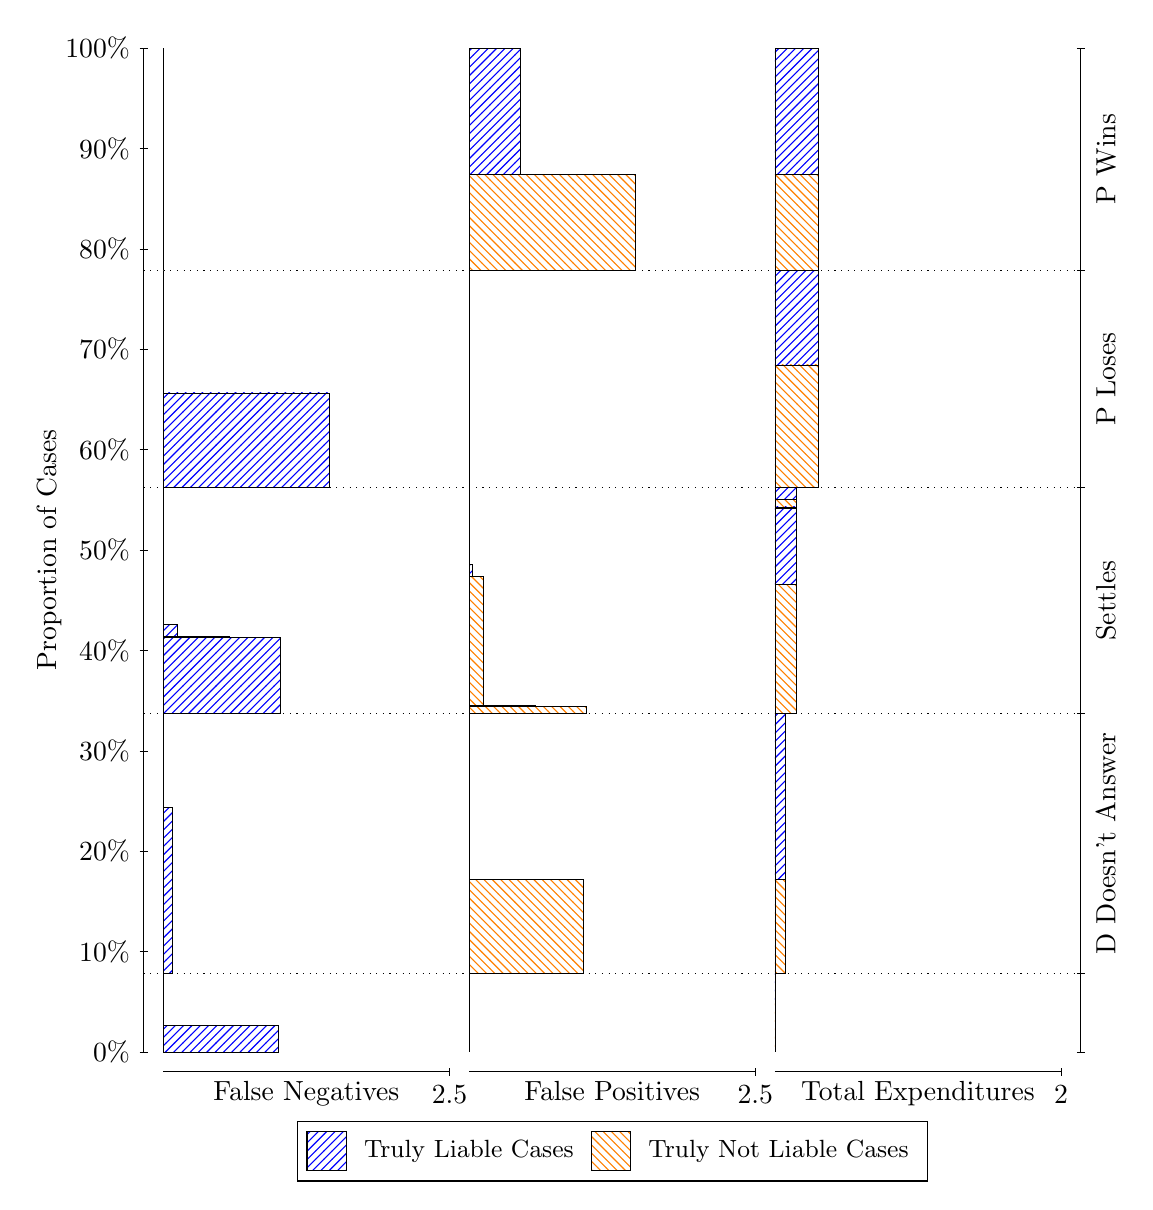
\begin{tikzpicture}
\draw[black, very thin] (1.5,1.75) -- (1.5,14.5);
\node[rotate=90, text=black, anchor=center] at (0.3, 8.125) {Proportion of Cases};
\draw[black, very thin] (1.45,1.75) -- (1.55,1.75);
\node[text=black, anchor=east] at (1.45, 1.75) {0\%};
\draw[black, very thin] (1.45,3.025) -- (1.55,3.025);
\node[text=black, anchor=east] at (1.45, 3.025) {10\%};
\draw[black, very thin] (1.45,4.3) -- (1.55,4.3);
\node[text=black, anchor=east] at (1.45, 4.3) {20\%};
\draw[black, very thin] (1.45,5.575) -- (1.55,5.575);
\node[text=black, anchor=east] at (1.45, 5.575) {30\%};
\draw[black, very thin] (1.45,6.85) -- (1.55,6.85);
\node[text=black, anchor=east] at (1.45, 6.85) {40\%};
\draw[black, very thin] (1.45,8.125) -- (1.55,8.125);
\node[text=black, anchor=east] at (1.45, 8.125) {50\%};
\draw[black, very thin] (1.45,9.4) -- (1.55,9.4);
\node[text=black, anchor=east] at (1.45, 9.4) {60\%};
\draw[black, very thin] (1.45,10.675) -- (1.55,10.675);
\node[text=black, anchor=east] at (1.45, 10.675) {70\%};
\draw[black, very thin] (1.45,11.95) -- (1.55,11.95);
\node[text=black, anchor=east] at (1.45, 11.95) {80\%};
\draw[black, very thin] (1.45,13.225) -- (1.55,13.225);
\node[text=black, anchor=east] at (1.45, 13.225) {90\%};
\draw[black, very thin] (1.45,14.5) -- (1.55,14.5);
\node[text=black, anchor=east] at (1.45, 14.5) {100\%};

\draw[black, very thin] (13.4,1.75) -- (13.4,14.5);
\draw[black, very thin] (13.35,1.75) -- (13.45,1.75);
\node[anchor=west] at (13.35, 1.75) {};
\draw[black, very thin] (13.35,2.7449) -- (13.45,2.7449);
\node[anchor=west] at (13.35, 2.7449) {};
\draw[black, very thin] (13.35,6.0481) -- (13.45,6.0481);
\node[anchor=west] at (13.35, 6.0481) {};
\draw[black, very thin] (13.35,8.9185) -- (13.45,8.9185);
\node[anchor=west] at (13.35, 8.9185) {};
\draw[black, very thin] (13.35,11.676) -- (13.45,11.676);
\node[anchor=west] at (13.35, 11.676) {};
\draw[black, very thin] (13.35,14.5) -- (13.45,14.5);
\node[anchor=west] at (13.35, 14.5) {};

\draw[black, very thin, pattern color=blue, pattern=north east lines] (1.75,1.75) rectangle (3.2033,2.0858);
\draw[black, very thin, pattern color=orange, pattern=north west lines] (1.75,2.0858) rectangle (1.75,2.7449);
\draw[black, very thin, pattern color=blue, pattern=north east lines] (1.75,2.7449) rectangle (1.859,4.853);
\draw[black, very thin, pattern color=orange, pattern=north west lines] (1.75,4.853) rectangle (1.75,6.0481);
\draw[black, very thin, pattern color=blue, pattern=north east lines] (1.75,6.0481) rectangle (3.2397,7.0178);
\draw[black, very thin, pattern color=blue, pattern=north east lines] (1.75,7.0178) rectangle (2.5857,7.025);
\draw[black, very thin, pattern color=blue, pattern=north east lines] (1.75,7.025) rectangle (1.9317,7.1764);
\draw[black, very thin, pattern color=orange, pattern=north west lines] (1.75,7.1764) rectangle (1.75,8.9185);
\draw[black, very thin, pattern color=blue, pattern=north east lines] (1.75,8.9185) rectangle (3.8573,10.119);
\draw[black, very thin, pattern color=orange, pattern=north west lines] (1.75,10.119) rectangle (1.75,11.676);
\draw[black, very thin, pattern color=orange, pattern=north west lines] (1.75,11.676) rectangle (1.75,12.898);
\draw[black, very thin, pattern color=blue, pattern=north east lines] (1.75,12.898) rectangle (1.75,14.5);
\draw[black, very thin, pattern color=orange, pattern=north west lines] (5.6333,1.75) rectangle (5.6333,2.4091);
\draw[black, very thin, pattern color=blue, pattern=north east lines] (5.6333,2.4091) rectangle (5.6333,2.7449);
\draw[black, very thin, pattern color=orange, pattern=north west lines] (5.6333,2.7449) rectangle (7.0867,3.94);
\draw[black, very thin, pattern color=blue, pattern=north east lines] (5.6333,3.94) rectangle (5.6333,6.0481);
\draw[black, very thin, pattern color=orange, pattern=north west lines] (5.6333,6.0481) rectangle (7.123,6.1413);
\draw[black, very thin, pattern color=orange, pattern=north west lines] (5.6333,6.1413) rectangle (6.469,6.1486);
\draw[black, very thin, pattern color=orange, pattern=north west lines] (5.6333,6.1486) rectangle (5.815,7.7902);
\draw[black, very thin, pattern color=blue, pattern=north east lines] (5.6333,7.7902) rectangle (5.6697,7.9417);
\draw[black, very thin, pattern color=blue, pattern=north east lines] (5.6333,7.9417) rectangle (5.6333,8.9185);
\draw[black, very thin, pattern color=orange, pattern=north west lines] (5.6333,8.9185) rectangle (5.6333,10.475);
\draw[black, very thin, pattern color=blue, pattern=north east lines] (5.6333,10.475) rectangle (5.6333,11.676);
\draw[black, very thin, pattern color=orange, pattern=north west lines] (5.6333,11.676) rectangle (7.7407,12.898);
\draw[black, very thin, pattern color=blue, pattern=north east lines] (5.6333,12.898) rectangle (6.2873,14.5);
\draw[black, very thin, pattern color=orange, pattern=north west lines] (9.5167,1.75) rectangle (9.5167,2.4091);
\draw[black, very thin, pattern color=blue, pattern=north east lines] (9.5167,2.4091) rectangle (9.5167,2.7449);
\draw[black, very thin, pattern color=orange, pattern=north west lines] (9.5167,2.7449) rectangle (9.6529,3.94);
\draw[black, very thin, pattern color=blue, pattern=north east lines] (9.5167,3.94) rectangle (9.6529,6.0481);
\draw[black, very thin, pattern color=orange, pattern=north west lines] (9.5167,6.0481) rectangle (9.7892,7.6897);
\draw[black, very thin, pattern color=blue, pattern=north east lines] (9.5167,7.6897) rectangle (9.7892,8.6595);
\draw[black, very thin, pattern color=orange, pattern=north west lines] (9.5167,8.6595) rectangle (9.7892,8.6667);
\draw[black, very thin, pattern color=blue, pattern=north east lines] (9.5167,8.6667) rectangle (9.7892,8.6739);
\draw[black, very thin, pattern color=orange, pattern=north west lines] (9.5167,8.6739) rectangle (9.7892,8.7671);
\draw[black, very thin, pattern color=blue, pattern=north east lines] (9.5167,8.7671) rectangle (9.7892,8.9185);
\draw[black, very thin, pattern color=orange, pattern=north west lines] (9.5167,8.9185) rectangle (10.062,10.475);
\draw[black, very thin, pattern color=blue, pattern=north east lines] (9.5167,10.475) rectangle (10.062,11.676);
\draw[black, very thin, pattern color=orange, pattern=north west lines] (9.5167,11.676) rectangle (10.062,12.898);
\draw[black, very thin, pattern color=blue, pattern=north east lines] (9.5167,12.898) rectangle (10.062,14.5);
\draw[black, dotted] (1.5,2.7449) -- (13.4,2.7449);
\draw[black, dotted] (1.5,6.0481) -- (13.4,6.0481);
\draw[black, dotted] (1.5,8.9185) -- (13.4,8.9185);
\draw[black, dotted] (1.5,11.676) -- (13.4,11.676);
\draw[black, very thin] (1.75,1.5) -- (5.3833,1.5);
\node[text=black, anchor=north] at (3.5667, 1.5) {False Negatives};
\draw[black, very thin] (5.3833,1.45) -- (5.3833,1.55);
\node[text=black, anchor=north] at (5.3833, 1.45) {2.5};

\draw[black, very thin] (5.6333,1.5) -- (9.2667,1.5);
\node[text=black, anchor=north] at (7.45, 1.5) {False Positives};
\draw[black, very thin] (9.2667,1.45) -- (9.2667,1.55);
\node[text=black, anchor=north] at (9.2667, 1.45) {2.5};

\draw[black, very thin] (9.5167,1.5) -- (13.15,1.5);
\node[text=black, anchor=north] at (11.333, 1.5) {Total Expenditures};
\draw[black, very thin] (13.15,1.45) -- (13.15,1.55);
\node[text=black, anchor=north] at (13.15, 1.45) {2};


\node[text=black, centered, rotate=90] at (13.72, 4.3965) {D Doesn't Answer};
\node[text=black, centered, rotate=90] at (13.72, 7.4833) {Settles};
\node[text=black, centered, rotate=90] at (13.72, 10.297) {P Loses};
\node[text=black, centered, rotate=90] at (13.72, 13.088) {P Wins};

\draw (7.449999999999999,1.5) node[draw=none] (baseCoordinate) {};
\begin{scope}[align=center]
        \matrix[scale=0.5, draw=black, below=0.5cm of baseCoordinate, nodes={draw}, column sep=0.1cm]{
            \node[rectangle, draw, minimum width=0.5cm, minimum height=0.5cm, pattern color=blue, pattern=north east lines] {}; &
            \node[draw=none, font=\small, text=black] (B) {Truly Liable Cases}; &
            \node[rectangle, draw, minimum width=0.5cm, minimum height=0.5cm, pattern color=orange, pattern=north west lines] {}; &
            \node[draw=none, font=\small, text=black] (B) {Truly Not Liable Cases}; \\
            };
\end{scope}

\end{tikzpicture}
\end{document}